\chapter{F-engine design}
\label{chap:fengine}

The F-engine firmware development for this project was carried out using the graphical Simulink environment, leveraging blocks from the \gls{casper}\footnote{\url{https://casper.berkeley.edu/wiki/Main_Page}} framework. CASPER offers a library of pre-built modules for common DSP operations, such as FFTs, PFBs, and filtering, that can be easily combined to implement complex signal processing pipelines for radio astronomy applications.  
This methodology enables the design of digital architectures through functional blocks and visual connections, simplifying development compared to traditional hardware description languages such as VHDL or Verilog. The CASPER toolflow also includes a compilation process that translates the Simulink designs into synthesizable HDL code, which can then be implemented on \glspl{fpga}. Nevertheless, some custom HDL coding was necessary to implement specific functionalities not covered by existing CASPER blocks. 

This chapter details the design of the F-engine for the \gls{charts} telescope, covering the overall architecture, the digitization and channelization chain, spectral reordering, data transmission to the X-engine and generation of local oscillators for the mixers in the FDM stage. 

\section{F-engine requirements}
\label{sec:f_engine_architecture}

As described in \S\ref{sec:charts_digital_backend}, the CHARTS digital backend employs an FX correlator architecture, where the F-engine performs initial channelization of the digitized antenna signals multiplexed by the \gls{fdm} boards.  

The design specifications (as stated in the objectives) for the F-engine were established as follows:

\begin{itemize}
    \item Operate over a bandwidth of at least \SI{2366}{\mega\hertz}, covering the full band delivered by the FDM stage.  
    \item Quantize spectral outputs into a compact 4+4 bit format, representing the real and imaginary components of each frequency channel.  
    \item Internally generate local oscillators for the FDM mixers, using the \gls{rfsoc} DAC ports.  
    \item Provide high-throughput data transmission using a QSFP28 optical interface, supporting \SI{100}{\giga\bit\per\second} links.  
    \item Implement spectral reordering logic to discard non-useful channels (e.g., below \SI{300}{\mega\hertz} or in the guard regions between FDM sub-bands).  
\end{itemize}

These requirements shaped the architecture, and each design decision is discussed in the following sections.  

\newpage
\section{Digitization}
\label{sec:digitization}

\begin{figure}[h!]
\centering
\begin{minipage}{0.5\textwidth}
The digitization stage is implemented using the \gls{rfdc} block of the RFSoC4x2, configured to achieve the required bandwidth while enabling complex sampling. The ADC sampling frequency was set to \SI{4.9152}{\giga\hertz}, sufficient to cover the target \SI{2366}{\mega\hertz} bandwidth. A decimation factor of 2 reduces the data rate for subsequent stages while preserving the spectral content of interest, and an internal NCO at \SI{-1.2288}{\giga\hertz} shifts the band of interest to baseband, generating complex I/Q samples centered at 0 Hz.

The choice of complex I/Q sampling was motivated by hardware constraints. For real sampling, the RFDC could not provide a power-of-two number of parallel samples at the required rate (greater than twice the target bandwidth, i.e. \SI{4732}{\mega\hertz}). By using quadrature sampling, the effective processed bandwidth equals the sampling rate $\nu_s$, which was fixed at \SI{4915.2}{\mega\hertz}. After decimation by 2, the usable baseband bandwidth becomes $\nu_s/2=\SI{2457.6}{\mega\hertz}$, matching the CHARTS requirements. Figure \ref{fig:quadrature_sampling_rfdc} illustrates the frequency-domain behavior of the signal from the analog input to the output of the RFDC.

Since the system must simultaneously digitize 32 antennas, with 8 signals multiplexed per ADC, all converters available in the RFSoC4x2 are used. In particular, the dual tiles 224 and 226 were enabled and configured for quadrature sampling (see Figure \ref{fig:rfsoc_tiles}). Table \ref{tab:rfdc_config} summarizes the configuration parameters for each ADC.
\end{minipage}
\hfill
\begin{minipage}{0.45\textwidth}
\centering
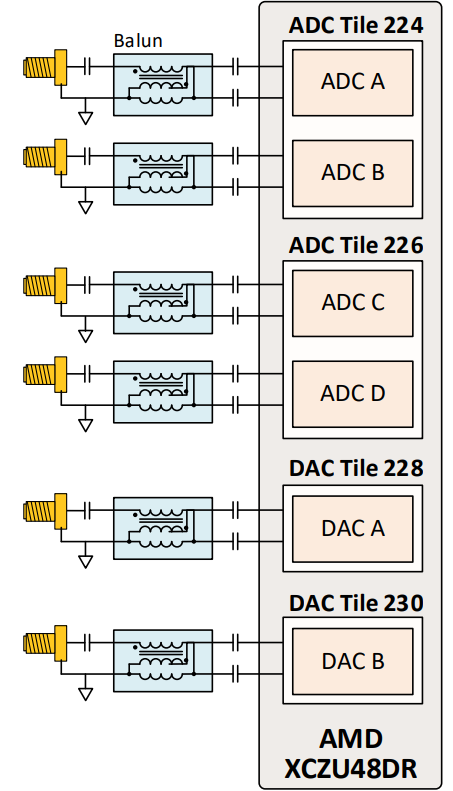
\includegraphics[width=0.9\textwidth]{rfsoc_tiles.png}
\caption[RFSoC4x2 ADC and DAC tiles]{RFSoC4x2 ADC and DAC tiles. The RFSoC4x2 contains 2 ADC and 2 DAC tiles. In this project, the dual ADC tiles 224 and 226 are used to digitize 8 antennas each, while the single DAC tile 228 generates the local oscillators for the FDM mixers.}
\label{fig:rfsoc_tiles}
\end{minipage}
\end{figure}

\begin{table}[h!]
\centering
\begin{tabular}{lc}
\toprule
Parameter & Value \\
\midrule
Sampling rate & 4915.2 Msps \\
Reference clock & 307.2 MHz \\
Digital Output & I/Q \\
Decimation Mode & 2x \\
Samples per Cycle & 8 \\
Mixer Type & Fine \\
Mixer Mode & Real $\rightarrow$ I/Q \\
NCO Frequency & $-1.2288$ GHz \\
NCO Phase & 0 \\
Nyquist Zone & Zone 1 \\
Calibration Mode & Mode 2 \\
\bottomrule
\end{tabular}
\caption{Configuration parameters of the RFSoC4x2 RFDC ADC dual tiles (224 and 226).}
\label{tab:rfdc_config}
\end{table}


With these configurations, the output data rate is \SI{256}{bits} per clock cycle, corresponding to 8 complex I/Q samples of \SI{32}{bits} each (16 + 16 signed), giving a required AXI4-Stream clock frequency of \SI{307.2}{\mega\hertz} to sustain the \SI{2457.6}{\mega\hertz} bandwidth. In order to produce this sample clock in the ADC tiles of the RFSoC, the Texas Instruments LMX2594 RF synthesizer was configured to generate a \SI{307.2}{\mega\hertz} reference, used by the ADC tile. This frequency is different from the \SI{491.52}{\mega\hertz} default reference clock provided in every CASPER image instance (\texttt{rfsoc4x2rfsoc4x2\_LMX\_REF\_245M76\_OUT\_491M52.txt} file), but due to harmonics of this clock appearing after channelization, it was changed to \SI{307.2}{\mega\hertz} so that the spurious tone falls exactly on an FFT bin, simplifying its removal in later stages.

Since for dual-tile platforms in I/Q digital output modes the in-phase and quadrature data are produced from different ports, before channelization the data stream is reordered using the CASPER \texttt{munge} block into the format $[I_1, Q_1, I_2, Q_2, \dots]$, ensuring compatibility with downstream processing blocks.

\begin{figure}[h!]
    \centering
    \includegraphics[width=\textwidth]{../figures/quadrature_sampling_rfdc.pdf}
    \caption[Illustration of the frequency-domain behavior of the signal across processing stages done by the RFDC]{Illustration of the frequency-domain behavior of the signal across processing stages done by the RFDC. The top panel shows the original analog signal obtained through FDM, occupying the first Nyquist zone between $0$ and $\nu_s/2$. The second panel corresponds to the digitized signal, where aliasing replicas appear both in the negative Nyquist zone ($-\nu_s/2$ to $0$) and in the second Nyquist zone ($\nu_s/2$ to $\nu_s$), as expected from sampling. The third panel illustrates the effect of mixing with a NCO at $-\nu_s/4$ (see Figure \ref{fig:quadrature_sampling}), which shifts the spectrum and redistributes its content symmetrically across the Nyquist regions. The bottom panel shows the result after decimation by a factor of two, where the spectrum is compressed into half the bandwidth, now spanning from $-\nu_s/4$ to $+\nu_s/4$.}
    \label{fig:quadrature_sampling_rfdc}
\end{figure}


\section{Channelization}
\label{sec:channelization}

Channelization is performed by a 4-tap PFB with convergent rounding and 18-bit coefficients. The output format of the PFB is set to 18 + 18 bits (real and imaginary parts), following CASPER design recommendations to balance precision and resource usage. 


The filtered samples are then passed to an 8192-point radix-2 pipeline FFT, which operates directly on the complex input.  The FFT is configured with automatic bit growth: at each stage of the 13-stage radix-2 pipeline, the word length increases by 1 bit to accommodate intermediate dynamic range expansion. Consequently, the final output has a format of $31 + 31$ bits, which is subsequently re-quantized according to the strategy described in \S\ref{sec:re-quantization}. As there are 13 stages the total number of channels is $2^{13} = 8192$, resulting in a channel width of \SI{300}{\kilo\hertz} over the \SI{2457.6}{\mega\hertz} bandwidth. The FFT is clocked at \SI{307.2}{\mega\hertz} with 8 samples per clock cycle, producing a new spectrum every \SI{3.33}{\micro\second}, and unlike real-input FFT architectures, no channels are discarded. 
Key specifications of the F-engine design are summarized in Table~\ref{tab:f_engine_metrics}.

The \SI{300}{\kilo\hertz} channel width provides the spectral resolution required for the intended scientific applications and mitigates dispersion-induced broadening (DM smearing), which is more acute in lower frequencies where the dispersion is greater. In addition, the \SI{3.33}{\micro\second} frame time resolution enables high-cadence, low-latency processing, facilitating calibration and correlation of antenna signals for each of the eight FDM chains. The full band and corresponding FFT bins for each chain are listed in Table~\ref{tab:fdm_chains}.
\begin{table}[htbp]
\centering
\begin{tabular}{l l}
\hline
Metric & Value \\
\hline
Frequency channels & 8192 \\
Effective bandwidth & \SI{2.4576}{\giga\hertz} \\
Channel width & \SI{300}{\kilo\hertz} \\
Frame time resolution & \SI{3.33}{\micro\second}  \\
\hline
\end{tabular}
\caption[F-engine specifications]{Key specifications of the F-engine design, including the number of frequency channels, effective bandwidth, channel width, and frame time resolution.}
\label{tab:f_engine_metrics}
\end{table}

\begin{table}[htbp]
\centering
\begin{tabular}{ccccc}
\toprule
Chain & Frequency Range & Bin Range & Number of Bins & Flipped \\
\midrule
0 & 300--499.8 MHz   & 1000--1666 & 667 & No \\
1 & 566--765.9 MHz   & 1887--2553 & 667 & Yes \\
2 & 833--1032.9 MHz  & 2777--3443 & 667 & Yes \\
3 & 1100--1299.9 MHz & 3667--4333 & 667 & Yes \\
4 & 1366--1565.7 MHz & 4553--5219 & 667 & No \\
5 & 1633--1832.7 MHz & 5443--6109 & 667 & No \\
6 & 1900--2099.7 MHz & 6333--6999 & 667 & No \\
7 & 2166--2365.8 MHz & 7220--7886 & 667 & No\\
\bottomrule
\end{tabular}
\caption[FDM chains and corresponding FFT bins]{FDM chains and corresponding FFT bins. Each of the 8 FDM chains covers a $\sim\SI{200}{\mega\hertz}$ band, with a \SI{66}{\mega\hertz} guard region between adjacent chains. The table lists the frequency range, FFT bin range, number of bins, and whether the spectrum is flipped due to mixing in FDM stage for each chain.}
\label{tab:fdm_chains}
\end{table}

\section{Re-quantization and calibration}
\label{sec:re-quantization}

\begin{figure}
    \centering
    \begin{tikzpicture}
	% Paths, nodes and wires:
	\node[shape=rectangle, minimum width=1.131cm, minimum height=0.631cm] at (5.983, 2.4){} node[anchor=center, align=center, text width=0.743cm, inner sep=6pt] at (5.983, 2.4){$g$};
	\node[mixer] at (6, 4){};
	\node[shape=rectangle, draw, line width=1pt, minimum width=1.215cm, minimum height=0.965cm] at (8.375, 4){} node[anchor=center, align=center, text width=0.827cm, inner sep=6pt] at (8.375, 4){$<<$};
	\draw[-latex] (6, 2.667) -- (6, 3.51);
	\node[shape=rectangle, minimum width=1.131cm, minimum height=0.631cm] at (4.75, 4.917){} node[anchor=center, align=center, text width=0.743cm, inner sep=6pt] at (4.75, 4.917){\small 31+31};
	\node[shape=rectangle, minimum width=0.765cm, minimum height=0.298cm] at (6.35, 3){} node[anchor=center, align=center, text width=0.377cm, inner sep=6pt] at (6.35, 3){\small 16};
	\node[shape=rectangle, minimum width=1.131cm, minimum height=0.631cm] at (7.25, 4.917){} node[anchor=center, align=center, text width=0.743cm, inner sep=6pt] at (7.25, 4.917){\small 48+48};
	\node[shape=rectangle, minimum width=0.565cm, minimum height=0.365cm] at (4.8, 3.8){} node[anchor=center, align=center, text width=0.177cm, inner sep=6pt] at (4.8, 3.8){\scriptsize 8};
	\node[shape=rectangle, minimum width=0.565cm, minimum height=0.365cm] at (7.2, 3.8){} node[anchor=center, align=center, text width=0.177cm, inner sep=6pt] at (7.2, 3.8){\scriptsize 8};
	\node[shape=rectangle, minimum width=1.131cm, minimum height=0.631cm] at (8.333, 2.167){} node[anchor=center, align=center, text width=0.743cm, inner sep=6pt] at (8.333, 2.167){dynamic\\shifter};
	\draw[-latex] (8.375, 2.657) -- (8.375, 3.5);
	\node[shape=rectangle, minimum width=0.565cm, minimum height=0.365cm] at (9.8, 3.8){} node[anchor=center, align=center, text width=0.177cm, inner sep=6pt] at (9.8, 3.8){\scriptsize 8};
	\node[shape=rectangle, draw, line width=1pt, minimum width=1.455cm, minimum height=0.765cm] at (11.255, 4){} node[anchor=center, align=center, text width=1.067cm, inner sep=6pt] at (11.255, 4){round};
	\node[shape=rectangle, minimum width=1.131cm, minimum height=0.631cm] at (9.75, 4.917){} node[anchor=center, align=center, text width=0.743cm, inner sep=6pt] at (9.75, 4.917){\small 48+48};
	\draw (4, 4) to[multiwire] (5.51, 4);
	\draw (6.49, 4) to[multiwire] (7.75, 4);
	\draw (9, 4) to[multiwire] (10.51, 4);
	\draw (12, 4) to[multiwire] (13.5, 4);
	\node[ocirc] at (13.5, 4){};
	\node[shape=rectangle, minimum width=0.565cm, minimum height=0.365cm] at (12.8, 3.8){} node[anchor=center, align=center, text width=0.177cm, inner sep=6pt] at (12.8, 3.8){\scriptsize 8};
	\node[shape=rectangle, minimum width=1.131cm, minimum height=0.631cm] at (12.667, 4.917){} node[anchor=center, align=center, text width=0.743cm, inner sep=6pt] at (12.667, 4.917){\small 4+4};
	\node[shape=rectangle, minimum width=0.765cm, minimum height=0.298cm] at (8.75, 3){} node[anchor=center, align=center, text width=0.377cm, inner sep=6pt] at (8.75, 3){\small 5};
	\node[shape=rectangle, draw, line width=1pt, minimum width=1.215cm, minimum height=0.965cm] at (3.375, 4){} node[anchor=center, align=center, text width=0.827cm, inner sep=6pt] at (3.375, 4){FFT};
\end{tikzpicture}
    \caption[Schematic of the quantization process]{Schematic of the quantization process. Gains can be configured independently for each channel, while the shift value is shared across all channels. After the left shift, convergent rounding to even is applied, keeping only the 4 most significant bits. This limits the representable range to $[-8,7]$. A clip flag is asserted whenever a value with an integer part equal to 0111 (decimal 7) and a non-zero fractional part reaches the rounding stage.}
    \label{fig:quantizer_architecture}
\end{figure}
\section{Spectral reordering}
\label{sec:spectral_reordering}


\section{Packetization and data transmission}

\label{sec:packetization}

\begin{table}[htbp]
\centering
\label{tab:packet_format}
\begin{tabular}{lll}
\toprule
\textbf{Field} & \textbf{Size (bytes)} & \textbf{Description} \\
\midrule
MCNT           & 8   & Monotonic counter, increments by 1 for each packet sent. \\
ADC ID         & 1   & Identifier of ADC source (0--3). \\
Num channels   & 2   & Number of frequency channels carried (8192). \\
Geometry ID    & 32   & Antenna/geometry index for array mapping\\
Flipped band & 1 & ID of FDM flipped bands (0111000) \\
Payload & 8192 & 8192 channels for each ADC.\\

\bottomrule
\end{tabular}
\end{table}

\section{LO generation}
\label{sec:lo_generation}